% ~ 3-4 pages
\chapter{Reconstruction, Energy Calibration and
  Identification of Hadronic Tau Lepton Decays}
\label{sec:reconstruction}

% TauBuilder config:
% https://gitlab.cern.ch/atlas/athena/blob/master/Reconstruction/tauRec/python/TauRecBuilder.py
%
% AlgHolders:
% https://gitlab.cern.ch/atlas/athena/blob/master/Reconstruction/tauRec/python/TauAlgorithmsHolder.py
%
This chapter describes the offline reconstruction of hadronic tau decays used in
the ATLAS experiment. It summarises the reconstruction as given in Refs.\
\cite{atlas:taurec:run1, atlas:taurec:run2}, while also including recent changes
to the reconstruction algorithms. The recent changes are compiled from
documentation available in the tau reconstruction packages of the ATLAS software
framework~\textsc{Athena}~\cite{athena}. The introduction of a track selection
and classification using multivariate methods in Ref.\ \cite{duschinger} has the
largest impact on the work presented in this thesis.

% JetSeedBuilder:
% https://gitlab.cern.ch/atlas/athena/blob/master/Reconstruction/tauRecTools/src/JetSeedBuilder.cxx
Candidates for hadronic tau decays are seeded by jets formed by the
anti-$k_\mathrm{t}$ jet algorithm using a distance parameter of $R = 0.4$ on
three-dimensional clusters of calorimeter cells called \emph{TopoClusters}. The
clusters are calibrated using the local hadronic calibration (LC) to account for
the non-compensating nature of the calorimeter, dead material and out-of-cluster
energy~\cite{local_hadronic_calib}. To seed a tau candidate the jet has to
satisfy~$p_\text{T} > \SI{10}{\GeV}$ and is required to fall into the acceptance
range of the tracking system~$|\eta| < \num{2.5}$.
% At this step tau $p_\mathrm{T}, \eta, \varphi, m$ ($m$: invariant mass) are
% set to the ones of the jet seed -- what does this mean? Read up on jet algs

\section{Vertex Association}
\label{sec:reco_vertex_assoc}
% TauVertexFinder:
% https://gitlab.cern.ch/atlas/athena/blob/master/Reconstruction/tauRecTools/src/TauVertexFinder.cxx
%
% Vertex association: Tracks matched unambiguously to jets via ghost-matching by
% adding all tracks into constituent list for the jet algorithm but setting
% their energy infinitesimally small (such that the result of the jet algorithm
% is not affected due to IR-safety) and rerunning the algorithm.
% \url{https://twiki.cern.ch/twiki/bin/view/AtlasProtected/JetGhostMatching}
%
% Tracking CP recommendations
% \url{https://twiki.cern.ch/twiki/bin/view/AtlasProtected/TrackingCPPreRecsSummer2017#Track_to_Vertex_Association}
In events with multiple primary vertices the tau production vertex has to be
identified. For this reconstructed tracks that are associated to the calorimeter
jet
% via ghost-matching\footnote{Tracks matched unambiguously to calorimeter jets
% by adding the tracks with infinitesimal energy to the constituent list
% and rerunning the jet algorithm.}
and lie in a cone of $\Delta R < 0.2$ with respect to the jet axis are selected.
Tracks that fulfil $p_\text{T} > \SI{1}{\GeV}$ and basic track quality
criteria\footnote{Number of pixel hits~$N_\text{Pixel} \geq 2$, number of
  silicon hits~$N_\text{Si} = N_\text{Pixel} + N_\text{SCT} \geq 7$. Dead
  sensors on the trajectory are also counted.} are used for vertex association.
The primary vertex maximising the so called \emph{Jet Vertex Fraction} (JVF)
\begin{align*}
  \text{JVF} = \frac{p_\text{T}\text{-sum of selected tracks assigned to the vertex}}{p_\text{T}\text{-sum of selected tracks}}
\end{align*}
% \begin{align*}
%   \mathrm{JVF} = \frac{\sum_\text{Vtx.\ \& TJVA} p_\mathrm{T}}
%                                            {\sum_\text{TJVA} p_\mathrm{T}}
% \end{align*}
is associated to the tau candidate.
% \footnote{Impact parameter based association with the
%   primary vertex. $|d_0| < \SI{2.5}{mm}$ with respect to beamline and
%   $|(\Delta z_0) \sin\theta| < \SI{3}{mm}$. $\Delta z_0$ is the longitudinal
%   distance of vertex and track}

% TauAxisSetter:
% https://gitlab.cern.ch/atlas/athena/blob/master/Reconstruction/tauRecTools/src/TauAxisSetter.cxx
After the primary vertex is found, the visible four-momentum of the tau
candidate is calculated.
% Assuming constituents have zero mass.
For this the barycentre of cluster energy (LC scale) in the jet is determined.
The four-momentum of each jet constituent in the coordinate system of the
associated vertex, falling within a cone of~$\Delta R < 0.2$ with respect to the
barycentre, is summed. This defines the visible tau momentum at LC scale and the
tau-axis. The visible tau momentum at LC scale is used as a baseline for further
energy calibrations.

\section{Track Selection and Classification}
\label{sec:reco_track_sel_classif}
% TauTrackFinder:
% https://gitlab.cern.ch/atlas/athena/blob/master/Reconstruction/tauRecTools/src/TauTrackFinder.cxx
%
% TauTrackClassifier:
% https://gitlab.cern.ch/atlas/athena/blob/master/Reconstruction/tauRecTools/Root/TauTrackClassifier.cxx
Tracks reconstructed in the inner detector are associated with a tau candidate
if they are within a cone of size~$\Delta R < 0.4$ with respect to the tau-axis.
% The tracks are classified into core, wide, and other tracks: If the tracks
% fail track selection (pt > 1GeV, IPd0Max = 1mm, IPz0Max = 1.5mm, nHitPix >= 2,
% nHitSi >= 7) they are classified as 'other'.
%
% If the tracks are within the 0.2 cone they are called 'core' tracks otherwise
% if they fall into the 0.2 - 0.4 annulus they are classified as 'wide'.
%
% Loose track selection for charged pions according to TrackingCP:
% pt > 400 MeV (This cut is already applied at track reco)
% |eta| < 2.5
% NSi >= 7
% N^sh_mod <= 1 (Number of shared models = N^sh_Pix + N^sh_SCT / 2)
% N^hole_Si <= 2
% N^hole_Pix <= 1
%
% Dirk's talk in TauCP:
% https://indico.cern.ch/event/615208/contributions/2481630/attachments/1415563/2167141/TauCP_TrackClassificationTaskforce_20170220.pdf
For each track a multi-class classification is performed categorising them into
one of four track-categories: \emph{charged}, \emph{conversion},
\emph{isolation} and \emph{fake}. Tracks classified as \emph{charged} are tracks
originating from charged pions of the tau decay. \emph{Conversion} tracks are
created by long-lived secondary particles from converted photons or hadronic
interactions. \emph{Isolation} tracks are from primary particles not originating
from the tau decay and \emph{fake} tracks from combinations of unrelated space
points in the inner detector.

The multi-class classification is performed by using three boosted decision
trees~(BDT) organised into two layers. In the first layer a single BDT performs
binary classification of tracks into one of two preliminary categories:
charged/conversion and isolation/fake. The second layer uses two BDTs to
separate the preliminary categories into the four final track-categories. The
BDTs employ information on track momentum, impact parameters, number of hits in
the ID, high-threshold hits in the TRT, etc.

The track classification is used to reconstruct the charge of the tau by summing
the charge of all \emph{charged} tracks. The number of \emph{charged} tracks
also defines whether the reconstructed tau is a 1- or 3-prong decay. This
algorithm is optimised to reconstruct taus with the correct number of
\emph{charged} tracks, such that the reconstruction efficiency is maximised.
Analyses often require reconstructed taus to have one or three \emph{charged}
tracks leading to a significant reduction in tau candidates originating from
multijet events due to their large track multiplicity. Using the \emph{charged}
classification a derived track-category is defined to calculate isolation
variables. The \emph{modified isolation} category consists of tracks not
classified as \emph{charged} and passing track selection criteria:
\begin{align*}
  &p_\text{T} > \SI{1}{\GeV} & &d_0^\text{PV} < \SI{1}{mm} & &|z_0^\text{PV} \sin\theta| < \SI{1.5}{mm} \\
  &N_\text{Pixel} \geq 2 & &N_\text{Si} \geq 7 \eqcomma
\end{align*}
where $d_0^\text{PV}$ ($z_0^\text{PV}$) is the transverse (longitudinal) impact
parameter with respect to the associated primary vertex and $N_\text{Pixel}$
($N_\text{Si}$) the number of pixel (silicon) hits including dead sensors on the
trajectory. Tracks in the \emph{modified isolation} category are used to
calculate discriminants, e.g.\ the momentum fraction of isolation tracks, for
tau-identification.

% \begin{figure}[htb]
%   \centering
%   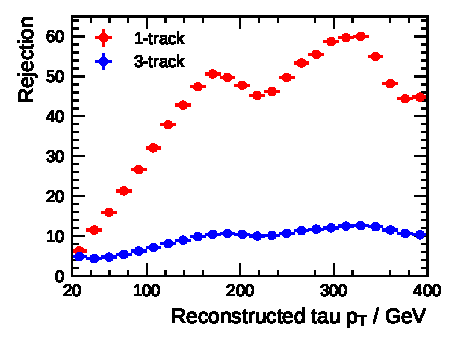
\includegraphics{./figures/bdt_perf/mva_tracking_rejection.pdf}
%   \caption{Rejection due to MVA tracking. Rejection of tau candidates from
%     dijets after baseline tau selection.}
%   \label{fig:mva_tracking_rejection}
%   \todo[inline]{Ticks are fucked. Increasing rejection with pt \textrightarrow
%     increasing multiplicity of jets with higher pt. Might be a problem with
%     weighting scheme?}
% \end{figure}

% Tau Tracks: tracks from the direct tau decay (pions)
%
% Conversion Tracks: tracks from conversions, hadronic interactions, 'long'
% living particles MVA Tracking input (barcode > 200k -- secondary particles)
%
% Isolation Tracks: mainly tracks from the underlying event (barcode < 10k but
% not tau tracks)
%
% Fake Tracks: not truth matched (10k < barcode < 200k) (includes pilup?)
%
% barcode < 200k -- primary particles
%
% variables: jetseed pt, track eta, z0SinThetaTJVA, rConvII, dRJetSeedAxis, d0,
% qOverP, nInnermostPixelHits, nPixelSharedHits, nSCTSharedHits, eProbabilityHT,
% nPixHits, nSiHits
% Impact params: reject conversion (d0), isolation and fake tracks (z0)
% Pixel, Si-Hits: rejection against conversions (missing hits)
% shared hits: intent is to recover merged tracks
% eProbabilityHT: Conversion tracks
% qOverP, dR: IT, FT

\section{Energy Calibration}
\label{sec:reco_energy_calib}
% TauCalibrateLC:
% https://gitlab.cern.ch/atlas/athena/blob/master/Reconstruction/tauRecTools/Root/TauCalibrateLC.cxx
%
% 5 eta bins: [0.0, 0.3, 0.8, 1.3, 1.6, 2.4]
% pile-up slopes for 1P and 3P for each eta bin
% mean pile-up for 1P and 3P
% A calibration function for 1P and 3P for each bin
%
% Offset calculated as
% offset = slope * (reco. num of PU vertices - average number of PU vertices)
% energyLC = ptDetectorAxis()
% if energyLC - offset <= 0: set offset to 0
% energyPUCorr = energyLC - offset
% calibConst = func(nProng, eta; energyPUCorr)
% if calibConst <= 0: calibConst = 1.0
% energyFinal = energyPUCorr / calibConst
%
The visible momentum measurement of the tau decay at LC scale is not optimised
to accurately reflect the true visible momentum. Additional corrections for
energy contributions due to pile-up, energy depositions outside of the
$\Delta R < 0.2$ cone and detector responses in different regions need to be
taken into account. Therefore, an energy calibration is applied to the
reconstructed object to reduce bias and improve the resolution of the energy
measurement.

The visible transverse momentum at LC scale~$p_\text{T}^\text{LC}$ increases
linearly with the number of reconstructed vertices~$N_\text{PV}$. Therefore, the
pile-up contribution to the transverse momentum is estimated
by~\cite{atlas:taurec:run2, calo_tes}
\begin{align*}
  p_\text{T}^\text{pileup}(N_\text{PV}, |\eta|, n_\text{p}) &= A(|\eta|, n_\text{p}) \times N_\text{PV} \eqcomma
\end{align*}
where $A$ is the average pile-up contribution per reconstructed vertex,
parametrised in bins of~$|\eta|$ and separately for 1- and multi-prong
decays~$n_\text{p}$.
% A is roughly of the order of 0.1 GeV per vertex
Subsequently, the momentum is corrected for the detector response to obtain the
visible transverse momentum at the tau energy scale~\cite{atlas:taurec:run2,
  calo_tes}
\begin{align*}
  p_\text{T}^\text{TES} &= \frac{p_\text{T}^\text{LC} - p_\text{T}^\text{pileup}}
                          {\mathcal{R}\left(p_\text{T}^\text{LC} - p_\text{T}^\text{pileup}, |\eta|, n_\text{p}\right)} \eqcomma
\end{align*}
with the detector response~$\mathcal{R}$, which is a function of the transverse
momentum after pile-up subtraction. The detector response is computed using a
fit of an empirical function to Gaussian means of
the~\mbox{$(p_\text{T}^\text{LC} - p_\text{T}^\text{pileup}) / p_\text{T,
    vis}^\text{true}$} distribution in different
$p_\text{T}^\text{LC} - p_\text{T}^\text{pileup}$ bins. The response
function~$\mathcal{R}$ is determined in five bins of $|\eta|$ and separately for
1- and multi-prong decays. More sophisticated energy calibrations for hadronic
tau decays exist, further improving the energy resolution. They are not
discussed here, as only LC- and TES-calibrated taus are used in this thesis.

\section{Shot Reconstruction}
\label{sec:shot_reco}

Reconstructing individual photons originating from neutral pions in hadronic tau
decays can be useful for various applications (e.g.\ classification of the
hadronic decay mode). The photons from the $\pi^0$-decay are highly collimated
and therefore deposit their energy in a single \emph{TopoCluster}. The fine
$\eta$-segmentation of the strip layer EM1 allows individual photons to be
detected using local maxima of cell energy. The reconstructed objects are called
\emph{shots}.

% TauShotFinder
% https://gitlab.cern.ch/atlas/athena/blob/master/Reconstruction/tauRecTools/src/TauShotFinder.cxx
The reconstruction of shots uses calorimeter cells in EM1 in a cone
of~$\Delta R < 0.4$ with respect to the tau-axis that
fulfil~$E_\text{T} > \SI{100}{\MeV}$. A shot is seeded by cells with a local
maximum of transverse energy in $\eta$.
% The neighboring cells are required to have smaller $E_\text{T}$.
If multiple seed cells are adjacent in~$\varphi$, the seed is merged with the
neighboring cell of the largest transverse energy. In this case the
four-momentum of the shot is set by summing the transverse energies and forming
the $E_\text{T}$-weighted angular position of both cells. Otherwise the shot
four-momentum is set to the four-momentum of the seed cell.

The number of photons~$N_\text{photons}$ in a shot is determined by its
transverse energy. If the transverse energy of the shot exceeds a detector
region dependent threshold of \num{300} to \SI{430}{\GeV}, a single photon is
counted. Otherwise, no photon is counted to reduce contributions of shots not
originating from photons. For large transverse momenta of the neutral pion the
strip layer cannot resolve individual photons, therefore shots exceeding
transverse energies of \SI{10}{\GeV} are counted twice.
% Bins: ($0, 0.8, 1.39, 1.51, 1.8, \infty$)
% Thresholds: \{430 MeV, 300 MeV, crack, 330 Mev, 350 MeV\}

%%% Local Variables:
%%% mode: latex
%%% TeX-master: "mythesis"
%%% End:
